\documentclass{scrartcl}
\usepackage[utf8]{inputenc}
\usepackage{graphicx}
\title{Project: Network Visualization}
\subtitle{Client: Amazon Web Services \\\\\\\ Team: Quadcore Productions\\}
\author{Themba Mbhele 14007950\\ Moses Mayimela 14019702 \\ Hlengekile Jita 14077893 \\ Mpho Baloyi 14133670 \\Department of Computer Science, University of Pretoria}
\date{01 May 2016}
\begin{document}
\maketitle
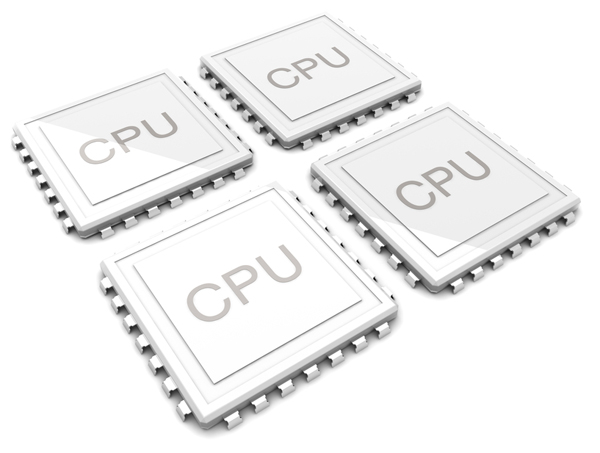
\includegraphics[width=\textwidth]{2012-quad-core-phones}
\section{The Team}
\subsection{Moses Mayimela}
\subsection{Hlengekile Jita}
\subsection{Mpho Baloyi}
\subsubsection{Interests}
\begin{itemize}
\item Keeping abreast with new technologies
\item Learning and using new technologies to solve problems
\item Reading up and doing research on new and old concepts in computer science
\item Solving riddles and puzzles
\item Helping people through ICT
\end{itemize}
\subsubsection{Technical Skills}
\begin{itemize}
\item Solid programming skills in java,c++ and python
\item Fair amount of knowlegde in assembly programming
\item Web development with HTML,JAVASCRIPT,JQUERY,CSS,PHP,AJAX,ANGULARJS
\item Interaction Design
\item Database design with MySQL
\item Understanding of process development
\item Unit testing,mocking and dependency Injection
\end{itemize}
\subsubsection{Non-technical Skills}
\begin{itemize}
\item Exellent Communication skills
\item Patient
\item Creative approach to problem solving
\item Pay attention to detail
\item Excellent planning skills
\item Ability to grasp concepts quickly
\item Willness to learn new things
\item Ability to interpret and follow technical plans
\item Ability to collaborate and work efficiently with other people
\item Ability to work under pressure
\end{itemize}
\subsubsection{What makes you want to do the project}
\begin{flushleft}
My interest and deep passion for Internet of Things,helping people and more importantly providing people with means to take
care of the enviroment through careful power consumption are the main reasons why I want to do this project. I also want to do
this project because it is an opportunity to learn and see how software and hardware work togther which has always been one of my many interests.The project presents an opportunity to learn new things,acquire new skills and refine my skills and I believe this is the headstart i need for my career in Computer Science.
\end{flushleft}
\subsection{Themba Mbhele}
\section{Project Execution}
\subsection{Development Methodology}
\subsection{Communication With Client}
\subsection{Technical Challenges}
\begin{itemize}
\item Learning the EC2 API 

As this is a very specific technology and one that we have not encountered before but we have a strong believe that 
through more research,more information from the client and our previous experiences with using an API we can overcome this challenge.

\item Retrieving Data from Amazon

This challenge is only due to the lack of information at this stage we plan to overcome this challenge by using either xml or JSON.
\end{itemize}
\subsection{Technologies}
\end{document}